
% This LaTeX was auto-generated from MATLAB code.
% To make changes, update the MATLAB code and republish this document.

\documentclass{article}
\usepackage{graphicx}
\usepackage{color}

\sloppy
\definecolor{lightgray}{gray}{0.5}
\setlength{\parindent}{0pt}

\begin{document}

    
    
\subsection*{Contents}

\begin{itemize}
\setlength{\itemsep}{-1ex}
   \item Part 1
   \item Part 2
\end{itemize}
\begin{verbatim}
% Feb 16, 2018
% Brian Hosler & Sarah Peachey
% Assignment 4
clear
close all
clc
\end{verbatim}


\subsection*{Part 1}

\begin{par}
extract the metadata tag associated with image   1) reading the quatization tables used to encode and decode in the   jpeg header   2) compare to list of digital camera models Need wine to use JPEGsnoop.exe :(
\end{par} \vspace{1em}


\subsection*{Part 2}

\begin{verbatim}
im1=imread('Assignment4Files/blockArtifacts1.tif');
k1=blockDetect(im1)

im2=imread('Assignment4Files/blockArtifacts2.tif');
k1=blockDetect(im2)

im3=imread('Assignment4Files/blockArtifacts3.tif');
k1=blockDetect(im2)

type('blockDetect.m')
\end{verbatim}

        \color{lightgray} \begin{verbatim}The strength of the blocking fingerprint is 1.498818e+00.
So the image was JPEG compressed 

k1 =

    1.4988

The strength of the blocking fingerprint is 1.496792e+00.
So the image was JPEG compressed 

k1 =

    1.4968

The strength of the blocking fingerprint is 1.496792e+00.
So the image was JPEG compressed 

k1 =

    1.4968


function [ k ] = blockDetect( im )
%blockDetect implements the Fan and de Quieroz?s JPEG blocking artifact
    % detecting algorithm. inputs any image and output the k, blcoking 
    % strength value. 
    Zp=[]; 
    Zpp=[];
    [r,c]=size(im); 
    for i=1:8:r-8 % dont do the last 8x8 block in row or cols 
        for j=1:8:c-8
            grid=im(i:i+7,j:j+7); % grid plus one 
            A=grid(4,4); 
            B=grid(4,5); 
            C=grid(5,4); 
            D=grid(5,5); 
            Zp=[Zp, double(abs(A-B-C+D))]; 
            E=grid(8,8); 
            F=im(i+7,i+8); 
            G=im(i+8,i+7); 
            H=im(i+8,i+8); 
            Zpp=[Zpp, double(abs(E-F-G+H))]; 
        end 
    end 
    % 2)
    figure 
    HI=histogram(Zp,255); 
    HI.Normalization = 'probability'; 
    hold on 
    HII=histogram(Zpp,255); 
    HII.Normalization = 'probability'; 
    legend('Normalized center values','Normalized edge values')
    % 3)
    k=sum(abs(HI.Values-HII.Values)); 
    n=0.25; 
    % 4) 
    jpegDetect = (k>n); 
    fprintf('The strength of the blocking fingerprint is %d.\n',k); 
    if jpegDetect==1
        fprintf('So the image was JPEG compressed \n')
    else
        fprintf('So the image was not JPEG compressed \n')
    end

end

\end{verbatim} \color{black}
    
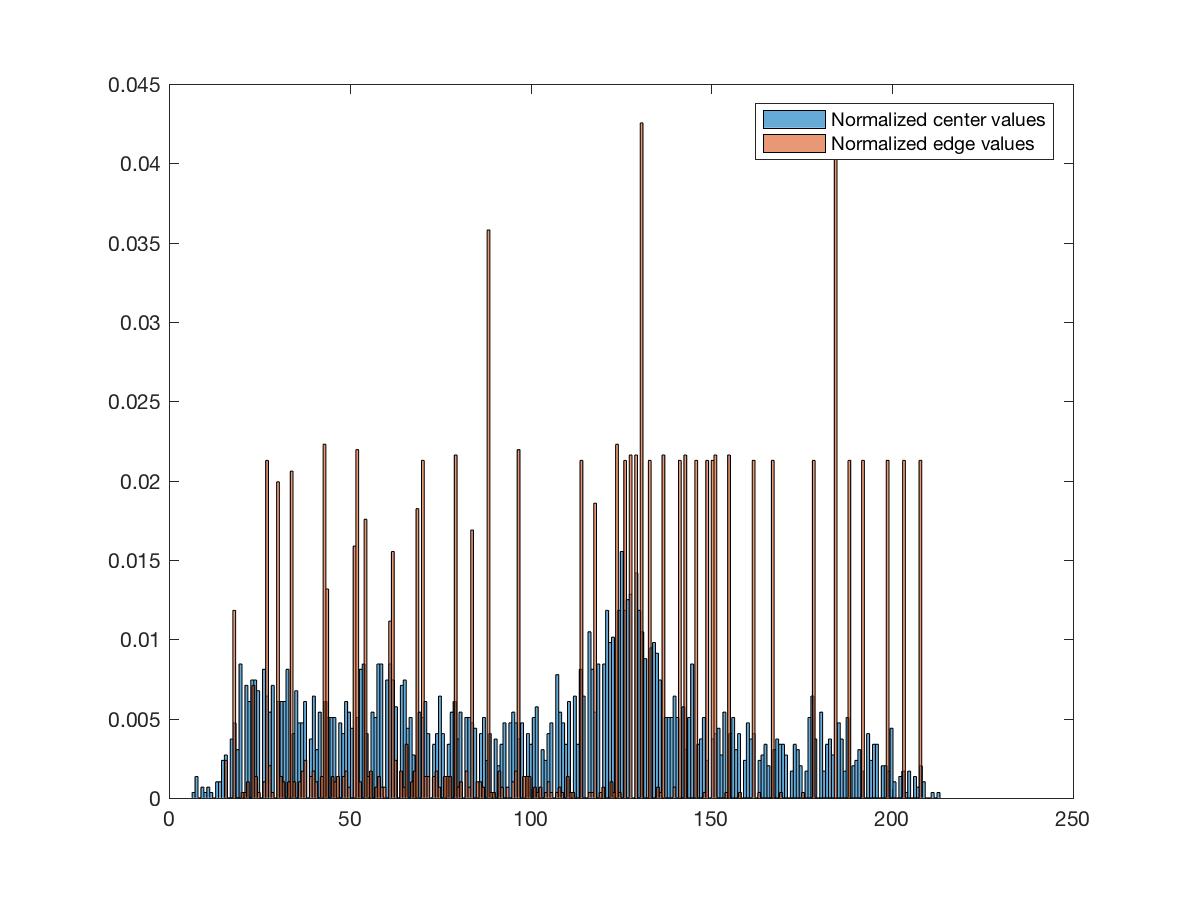
\includegraphics [width=4in]{lab4_01.eps}

\includegraphics [width=4in]{lab4_02.eps}

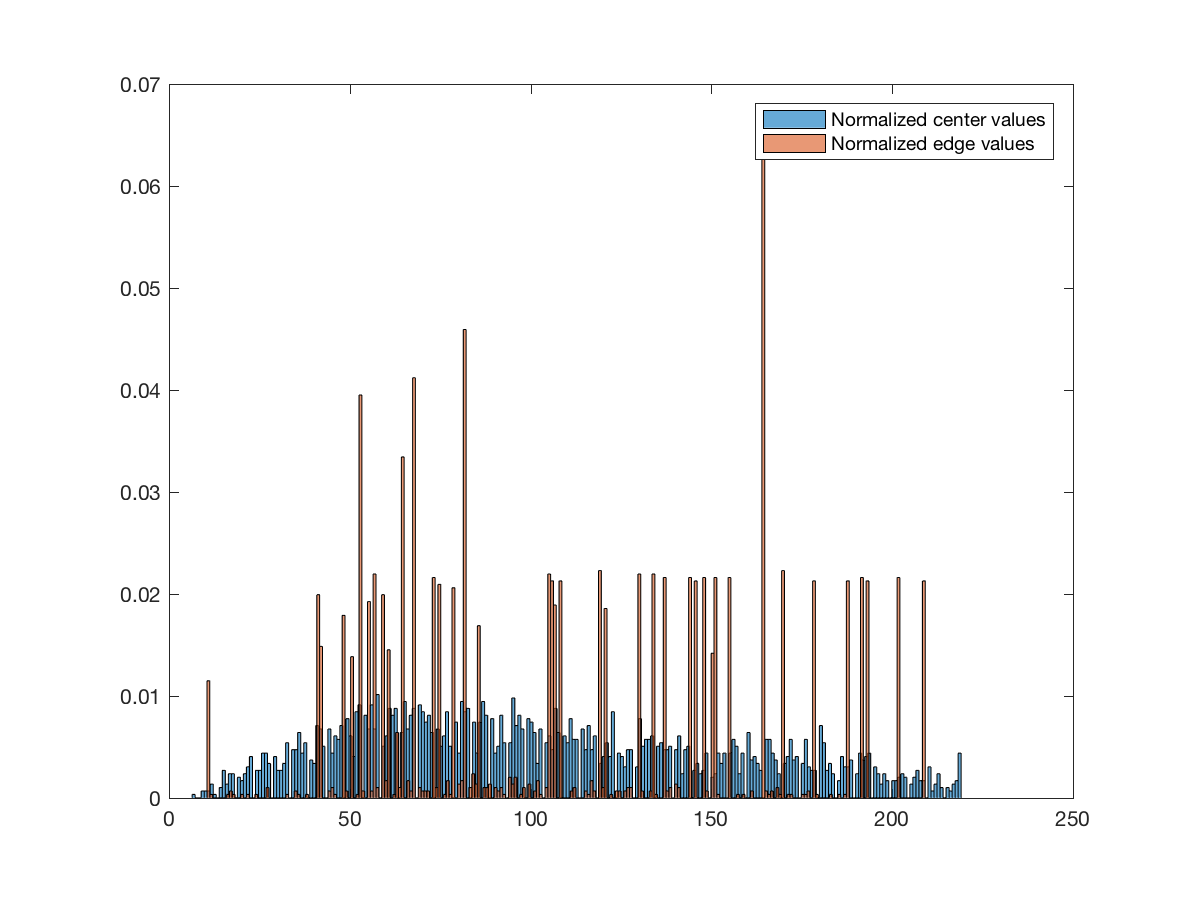
\includegraphics [width=4in]{lab4_03.eps}



\end{document}
    
